\chapter{Aspectos de diseño y desarrollo}
\label{chapter:disenyo_y_desarrollo}


%%% SECTION
\section{Aspectos de diseño}
El planteamiento inicial de este proyecto, en lo que se refiere al diseño, fue realizarlo íntegramente en el entorno de \textit{``Big Data"} Azure HDInsight.
Puesto que este entorno todavía tiene carencias por estar en una fase temprana de despliegue, nos hemos apoyado también en el entorno ``Databricks Community Edition"\cite{databricks}, visto en el laboratorio de la asignatura de ``Análisis de datos en entornos Big Data".

A continuación describiremos las distintas fases que se van a realizar a lo largo del desarrollo del proyecto.

\subsection{Estudio preliminar}
Esta fase va a ser el punto de partida para el resto del trabajo, vamos a tratar de entender el negocio así como la intención de los retos propuestos.
Además, focalizaremos nuestra atención en la comprensión de los datos y la determinación de los requerimientos de información necesarios para poder llevar a cabo nuestro proyecto.

\subsection{Tratamiento y saneamiento de los datos}
Una vez los recursos de datos están identificados, es necesario que sean seleccionados, limpiados, transformados a la forma deseada y formateados. En esta fase se llevará a cabo los procesos de transformación y limpieza de datos, necesarios para el posterior modelado.
Como partimos de unos datos que ya están cargados en el almacenamiento del cluster de Big Data, no tendremos que preocuparnos por la carga de estos desde otros sistemas.
El objetivo de esta fase será, conseguir varias tablas enriquecidas con la información otras tablas para que luego nos sirva para entrenar nuestro modelo y obtener predicciones.
Es por esto que tendremos que seleccionar los atributos que veamos que pueden ser interesantes a la vez que crear datos agregados que puedan suponer un valor añadido.
Por otra parte, deberemos sanear esos datos para luego facilitar las fases de creación y entrenamiento de los modelos predictivos. Estas tareas de adecuación las podemos agrupar en: tareas de limpieza, normalización, discretización y reducción de la dimensionalidad.  

\begin{enumerate}
    \item Limpieza de datos:
    
En este proceso se llevan a cabo actividades de detección, eliminación o corrección de valores inapropiados en el conjunto de datos. Se pretende detectar y subsanar los errores de forma que obtengamos unos datos lo más completos y consistentes posible.

    \item Normalización de datos:
    
En la normalización de datos trataremos de lograr que los datos estén en una escala de valores equivalentes para simplificar la comparación entre ellos.

La normalización es útil para varios métodos de minería de datos, de forma que reducimos la influencia de los atributos con valores más altos y que pueden distorsionr el resultado del modelo.


Existen varios métodos de normalización, como la normalización por el máximo, por la diferencia y por la desviación estándar.

    \item Discretización de datos:
    
    
En la discretización cambiaremos los valores de una variable continua en contenedores, intervalos o grupos, para limitar el número de estados posibles. 
De esta forma podremos tratar a los contenedores como si fueran categorías.
Los métodos de discretización se pueden clasificar en estas tres categorías:
\begin{itemize}
    \item Supervisados o no supervisados.
    \item Locales o globales.
    \item Parametrizados y no parametrizados.
\end{itemize}

    \item Reducción de la dimensionalidad:
    
En la reducción de la dimensionalidad reduciremos el número aleatorio de variables para obtener un conjunto de variables principales manteniendo el nivel de calidad necesario. Está dividido en dos tipos, selección de atributos y extracción de atributos.

\end{enumerate}

\subsection{Exploración y análisis de los datos}
La exploración y análisis de los datos o EDA (acrónimo  de \textit{``Exploratory Data Analysis"}) es importante y recomendada en los pasos previos al entrenamiento del modelo de \textit{``machine learning"}. Estas tareas se basan en el uso de cuadros resumen y herramientas gráficas que permiten detectar visualmente la distribución de los datos, la presencia de valores extremos y las relaciones entre los atributos.

\subsection{Creación y entrenamiento del modelo predictivo}
En esta sección, crearemos diferentes tipos de modelos para luego poder compararlos y elegir el que mejores resultados nos ofrezca o el que mejor se adapte a las condiciones de nuestro entorno.
Previamente a la creación del modelo dividiremos el conjunto de datos en dos bloques, uno para entrenar el modelo y otro para validar la precisión de los resultados.
De esta forma evitaremos que nuestro modelo se sobreentrene (en inglés, \textit{overfitting} y sea independiente de los datos utilizados en el entrenamiento.
Esto tiene sentido hacerlo porque nuestro modelo es de aprendizaje supervisado, para otros modelos que no son de este tipo no es necesario realizar esta división de los datos.

\subsection{Validación y visualización de los resultados}
Una vez tenemos nuestro modelo creado y entrenado pasaremos al último paso que es la validación. 
Con el otro conjunto de datos que no hemos utilizado para el entrenamiento, lo usaremos para realizar las predicciones de forma que podamos comparar la predicción del modelo con el resultado real.

Para esta evaluación de los resultados nos apoyaremos de métricas e indicadores que puedan cuantificar la precisión del modelo, permitiendo la comparación entre distintos métodos sobre el mismo conjunto de datos.

Existen distintas métricas específicas para los problemas de clasificación, regresión o agrupamiento.
En nuestro caso vamos a tratar de problemas de clasificación, por lo que las métricas que usaremos será la matriz de confusión y otras métricas derivadas de esta.

\subsubsection{Matriz de confusión}
La matriz de confusión (confusion matrix) muestra gráficamente los aciertos y errores cometidos por el modelo de clasificación. 
\begin{figure}[H]
\centerline{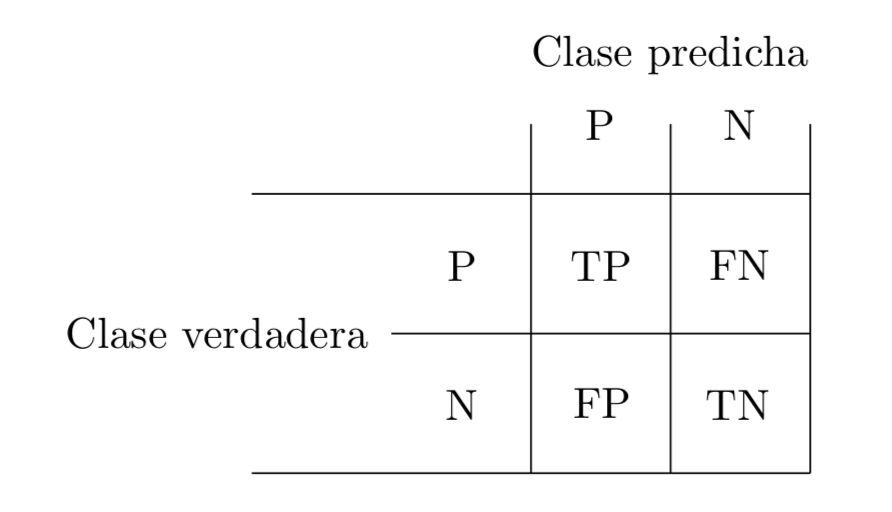
\includegraphics[width=0.5\textwidth]{TFM/figs/matrizconfusion.png}}
\caption{Matriz de confusión binaria}
\label{fig:matrizconfusion}
\end{figure}
Los parámetros que nos indica son:
Verdadero positivo (\textit{True Positive}, TP): número de clasificaciones correctas en la clase positiva (P).
Verdadero negativo (\textit{True Negative}, TN): número de clasificaciones correctas en la clase negativa (N).
Falso negativo (\textit{False Negative}, FN): número de clasificaciones incorrectas de clase positiva clasificada como negativa.
Falso positivo (\textit{False Positive}, FP): número de clasificaciones incorrectas de clase negativa clasificada como positiva.

\subsubsection{Métricas derivadas de la matriz de confusión}
A partir de la matriz de confusión, podemos obtener un conjunto de métricas que permiten cuantificar la bondad de un modelo de clasificación.
Podemos definir las siguientes:
\begin{itemize}
    \item Exactitud (\textit{accuracy}, ACC): número de predicciones correctas sobre el número total de predicciones.
    \begin{equation}
    ACC=\frac{TP+TN}{FP+FN+TP+TN}
    \end{equation}
    \item Error de clasificación (\textit{misclassification error}, ERR): número de predicciones incorrectas sobre el número total de predicciones.
    \begin{equation}
    ERR=\frac{FP+FN}{FP+FN+TP+TN}=1-ACC
    \end{equation}
    \item Tasa de verdaderos positivos (\textit{True Positive Rate}, TPR): tasa de acierto en los verdaderos positivos.
    \begin{equation}
    TPR=\frac{TP}{FN+TP}
    \end{equation} 
    \item Tasa de verdaderos negativos (\textit{False Positive Rate}, FPR): tasa de error en los falsos positivos.
    \begin{equation}
    FPR=\frac{FP}{FP+TN}
    \end{equation}
    \item Precisión (\textit{precision}, PRE): relaciona las tasas de verdaderos positivos y negativos.
    \begin{equation}
    PRE=\frac{TP}{FP+TP}
    \end{equation}
    \item Sensibilidad (\textit{recall}, REC): tasa de acierto en los verdaderos positivos.
       \begin{equation}
    REC=\frac{TP}{FN+TP}=TPR
    \end{equation}
    \item Especificidad (\textit{specificity}, SPE): tasa de instancias correctamente clasificadas como negativas respecto a todas las instancias negativas.
    \begin{equation}
    SPE=\frac{TN}{FP+TN}=1-FPR
    \end{equation}
    \item F1 (\textit{F1 score}): combina la precisión y la sensibilidad.
    \begin{equation}
    F1=2\times\frac{PRE \times REC}{PRE+REC}
    \end{equation} 
    
\end{itemize}

\subsubsection{Curva ROC}
Una curva ROC (acrónimo de \textit{Receiver Operating Characteristic}) mide el rendimiento respecto a los falsos positivos (FP) y verdaderos positivos (TP).
\begin{figure}[H]
\centerline{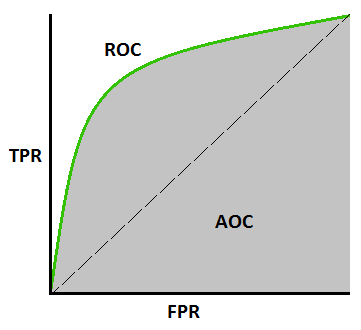
\includegraphics[width=0.5\textwidth]{TFM/figs/roc.png}}
\caption{Curva ROC}
\label{fig:roc}
\end{figure}

En esta métrica, se puede ver que cuanto más pegada esté la curva a la esquina superior izquierda del gráfico mejor clasificador será.

A partir de esta curva, podemos calcular el área bajo la curva (\textit{area under the curve}, AUC) que muestra el rendimiento del modelo de clasificación.



%%% SECTION
\section{Desarrollo}

En este apartado vamos a describir los pasos que hemos realizado para elaborar los objetivos que se plantearon al inicio del proyecto.

Todo el código fuente elaborado para el desarrollo de estos objetivos para se puede encontrar en el repositorio  \href{github}{https://github.com/dieconji/tfm/tree/master/code}.


\subsection{Análisis previo}
El objetivo principal era conocer qué funcionalidades en las plataformas digitales permiten la reducción de llamadas telefónicas recibidas.

Tras analizar los datos disponibles, se ha tomado la decisión de dividir este objetivo principal en dos modelos, de forma que con la ayuda de estos dos seamos capaces de obtener el conocimiento que se sugiere en la misión principal.
El motivo de necesitar dividir este objetivo es porque con los datos que tenemos no se puede cuantificar la precisión de nuestro modelo, ya que los resultados finales no se pueden contrastar con la realidad si no la conocemos.

Así pues, los dos objetivos que vamos a plantear son los siguientes:
\begin{itemize}
    \item Predicción del canal por el que se ha realizado una reclamación:
    
    La misión de este modelo va a ser predecir si la reclamación que ha realizado un cliente ha sido por las plataformas digitales o por otros canales
    \item Predicción de facturación electrónica:
    
    Con este modelo podremos predecir, dado un cliente si tiene facturación electrónica o no.
\end{itemize}


\subsection{Creación de tablas minables}
Como nuestro objetivo es obtener dos modelos analíticos predictivos distintos, tenemos que plantearnos qué tipo de información vamos a necesitar para cada uno de ellos.

Así pues, tras estudiar el conjunto de datos y analizar los retos propuestos se ha decidido la creación de dos tablas minables distintas, creadas a partir de la información disponible, de modo que cada una de ella sirva para crear, entrenar y validar cada objetivo.
Estas tablas serán las siguientes:
\begin{itemize}
    \item Cliente: Cada registro pertenece a un cliente/contrato. Esta tabla está  enriquecida con información sobre su facturación, sobre las acciones que ha realizado en distintos canales y sobre sus sesiones en las plataformas digitales.
    \item Acción: Cada registro pertenece a una acción de tipo reclamación. Está enriquecida con la información del cliente, facturación del cliente y sesiones en las plataformas digitales.
\end{itemize}

Estas tablas van a compartir información en común, el inicio de creación de ambas tablas va a ser compartido pero el formato y características obliga a que se tengan que tomar varios caminos para la creación final de cada una.

Inicialmente se intentó generar esta información directamente desde el entorno Big Data con el uso de Zeppelin\cite{zeppelin}, pero ocasionó muchos problemas varios motivos:
\begin{itemize}
    \item Apagado automático del cluster los fines de semana:
    
    Por motivos económicos, los clusters de HDInsights estaban programados para eliminarse los fines de semana y volver a crearse el lunes a primera hora. Esto es una de las ventajas de los entornos cloud de Big Data, pero que nos ha ocasionado más problemas de los previstos inicialmente. 
    \item Fallos operativos en el entorno de \textit{notebooks} Zeppelin:
    
    Tras haber trabajado con los \textit{notebooks} de Jupyter\cite{jupyter} y Databricks, la idea de trabajar con Zeppelin parecía la más adecuada. Sin embargo, en esta instalación que disponíamos fallaba cada vez que se cancelaba una consulta, de forma que el servicio se quedaba bloqueado hasta que se reiniciara el servicio. El usuario que tenía disponible carecía de tales permisos, por lo que había que lanzar una incidencia y esperar que la tramitasen hasta varios días después.
\end{itemize}

Tras estos problemas iniciales se optó por trabajar con \textit{scripts Pyhton}\cite{python}. Además, como el tiempo de ejecución de la mayoría de las consultas era muy elevado, además de limitar el tamaño de las tablas para las pruebas iniciales, se utilizó la aplicación \textit{nohup}\cite{nohup} para poder dejar ``en ejecución" una consulta en \textit{background} y no depender de tener la sesión abierta.

De esta forma para cada operación de cruce entre tablas o enriquecimiento en el \textit{script} se modeló de la forma siguiente:
\begin{itemize}
    \item Insertar un registro en la tabla log de la BBDD con la fecha y título de la operación.
    \item Borrar tabla persistente en caso de existir.
    \item Crear un \textit{dataframe} a partir de la consulta SQL en la tabla.
    \item Crear una tabla temporal en la BBDD con la información del \textit{dataframe}.
    \item Crear una tabla persistente a partir de la temporal
\end{itemize}

Un ejemplo de código de una operación sería el siguiente:

\begin{minipage}{\linewidth}
\begin{lstlisting}[language=Python, caption=Ejemplo de operación en la creación de las tablas minables]
### FACTURAS
sqlContext.sql("insert into u257030.log select current_timestamp() fecha , 'FACTURAS' operacion")
facturas_df = sqlContext.sql("SELECT cod_cliente, cod_contrato, avg(imp_total_factu) as importe_medio FROM dwvp.ghh_factura GROUP BY cod_cliente, cod_contrato")
sqlContext.sql("DROP TABLE IF EXISTS u257030.facturas_df")
facturas_df.createOrReplaceTempView("tmp_facturas_df")
sqlContext.sql("CREATE TABLE u257030.facturas_df USING PARQUET AS SELECT * FROM tmp_facturas_df")
\end{lstlisting}
\end{minipage}  


Una vez obtenidas las tablas finales, enriquecidas con todos los campos que pueden aportar valor, las exportamos en ficheros CSV para poder tratarlas en Databricks. Como las tablas finales eran muy pesadas se hicieron descargas con registros limitados para hacer poder manejarlos de una manera más cómoda.

Todo el ciclo de vida del proyecto se pretendió gestionarlo íntegramente en el entorno HDInsight, pero dados los problemas detectados se consideró continuar el desarrollo en Databricks. De esta forma podríamos trabajar con un entorno notebook que nos permitiera trabajar de una forma mucho más ágil y cómoda que el entorno que se eligió en un inicio.

\subsection{Limpieza de datos}
Tras la importación de las tablas minables en Databricks se continuó con la limpieza de los datos.
Aquí primero se realizaron las siguientes procesos:
\begin{itemize}
    \item Tratar los valores vacíos o nulos:
    En el caso de campos categóricos añadiendo una nueva categoría con el valor 'NULO' y para los numéricos la media y la creación de un campo nuevo binario para indicar si era o no nulo.
    \item Normalizar las fechas:
    Se cambia de String/Timestamp a tipo Integer con el formato YYYYMMDD.
    \item Normalizar los campos numéricos a valores entre 0 y 1.
    \item Codificar las variables categóricas a columnas binarias con el método OneHotEncoder.
\end{itemize}

\subsection{Creación de los modelos}
Una vez ya tenemos los datos saneados podemos comenzar con la generación de modelos.

Para esto dividiremos nuestro \textit{dataset} en dos conjuntos, un 70\% para el entrenamiento y un 30\% para las validaciones.

Los modelos predictivos que se realizaron son en ambos casos de la tipología categorización, y fueron de los siguientes métodos:
\begin{itemize}
    \item Logistic Regression\cite{lr}.
    
La regresión logística es un método popular para predecir una respuesta categórica. Es un caso especial de los modelos \texit{`Generalized Linear models'} que predicen la probabilidad de las salidas. Este método puede ser usado tanto para predecir una salida binaria como para predecir una salida multiclase.

    \item Decision Tree Classifier\cite{dtc}.
    
Los árboles de decisión son unos métodos populares de la familia de clasificación y regresión.
Están ampliamente extendidos por su facilidad de interpretar, manejar características categóricas, extender a la clasificación multiclase, y son capaces de capturar no linealidades y interacciones de características.

    \item Random Forest Classifier\cite{rfc}.
    
Los clasificadores \textit{``Random Forests"} son conjuntos de árboles de decisión, cominándolos de forma que se reduce el riesgo de sobreentreamiento.

    \item Gradient-boosted Tree Classifier\cite{gbt}.
    
Los clasificadores \textit{``Gradient-boosted Tree"} entrenan iterativamente árboles de decisión en orden de minimizar la función de pérdida o \textit{``loss"}.

    \item Linear Support Vector Machine\cite{lsvm}.
    
Una máquina de soporte vectorial construye un hiperplano o conjunto de hiperplanos en un espacio de dimensiones muy altas o infinitas que pueden ser usadas para tareas de clasificación, regresión, u otras tareas. Instintivamente, una buena separación se consigue por el hiperplano que tiene mayor distancia a los puntos más cercanos de los datos de entreamiento de cualquier clase, en general, a mayor margen menor error de generalización del clasificador.

\end{itemize}

Para cada uno de ellos, el procedimiento de creación, entrenamiento y generación de predicciones ha sido el mismo.
Este es un ejemplo de cómo se ha generado el modelo de Gradient-boosted Tree Classifier:

\begin{minipage}{\linewidth}
\begin{lstlisting}[language=Python, caption=Métricas derivadas de la matriz de confusión]
from pyspark.ml.classification import GBTClassifier

# creamos el modelo
gbt = GBTClassifier(maxIter=10)

# entrenamos el modelo
gbtModel = gbt.fit(train)

# obtenemos las predicciones del conjunto test
predictions = gbtModel.transform(test)
\end{lstlisting}
\end{minipage}  

Por último, para poder medir la calidad de cada modelo nos hemos ayudado de los siguientes elementos:

\begin{itemize}
\begin{minipage}{\linewidth}
    \item Matriz de confusión

\begin{lstlisting}[language=Python, caption=Matriz de confusión]
from sklearn.metrics import confusion_matrix

def matriz_confusion(y_true, y_pred):
  # nombre de las clases
  class_names = [0, 1]

  # creamos matriz de confusion
  cnf_matrix = confusion_matrix(y_true, y_pred, labels=class_names)
  
  # normalizamos
  cm = cnf_matrix.astype('float') / cnf_matrix.sum(axis=1)[:, np.newaxis]
  
  # mostramos matriz de confusion
  plt.imshow(cm, interpolation='nearest', cmap=plt.cm.Blues, aspect="auto")
  plt.title('Matriz de confusion normalizada')
  plt.colorbar()
  tick_marks = np.arange(len(class_names))
  plt.xticks(tick_marks, class_names, rotation=45)
  plt.yticks(tick_marks, class_names)

  thresh = cm.max() / 2.
  for i, j in itertools.product(range(cm.shape[0]), range(cm.shape[1])):
      plt.text(j, i, format(cm[i, j], '.2f'),
               horizontalalignment="center",
               color="white" if cm[i, j] > thresh else "black")

  plt.tight_layout()
  plt.ylabel('Clase verdadera')
  plt.xlabel('Clase predicha')
\end{lstlisting}
\end{minipage}  

\begin{minipage}{\linewidth}
    \item Métricas derivadas de la matriz de confusión

\begin{lstlisting}[language=Python, caption=Métricas derivadas de la matriz de confusión]
def mostrar_metricas(predictions):
  # devuelve las clases
  y_true = predictions.select("label")
  y_true = y_true.toPandas()

  # devuelve las predicciones
  y_pred = predictions.select("prediction")
  y_pred = y_pred.toPandas()

  # obtenemos la matriz de confusion
  TN, FP, FN, TP = confusion_matrix(y_true, y_pred).ravel()
  
  # cambiamos el tipo a float
  FP = FP.astype(float)
  FN = FN.astype(float)
  TP = TP.astype(float)
  TN = TN.astype(float)

  # obtenemos las metricas
  REC = TP/(TP+FN)
  SPE = TN/(TN+FP) 
  PRE = TP/(TP+FP)
  FPR = FP/(FP+TN)
  ACC = (TP+TN)/(TP+FP+FN+TN)
  ERR = 1-ACC
  F1 = 2*(PRE*REC)/(PRE+REC)
  evaluator = BinaryClassificationEvaluator()
  AUROC = evaluator.evaluate(predictions, {evaluator.metricName: "areaUnderROC"})
  
  # mostramos las metricas
  print('Exactitud (ACC): {:.2f}'.format(ACC))
  print('Error de clasificacion (ERR): {:.2f}'.format(ERR))
  print('Tasa de verdaderos positivos o sensibilidad (TPR | REC): {:.2f}'.format(REC))
  print('Tasa de verdaderos negativos (FPR): {:.2f}'.format(FPR))
  print('Precision (PRE): {:.2f}'.format(PRE))
  print('Especificidad(SPE): {:.2f}'.format(SPE))
  print('F1: {:.2f}'.format(F1))  
  print('Area bajo la curva ROC: {:.2f}'.format(AUROC))
\end{lstlisting}
\end{minipage}

\begin{minipage}{\linewidth}
    \item Curva ROC

\begin{lstlisting}[language=Python, caption=Curva ROC]
from sklearn.metrics import roc_curve  

def curva_roc(y_true, y_pred):
  # obtenemos ratio de falsos positivos y verdaderos positivos
  fpr, tpr, thresholds = roc_curve(y_true, y_pred)

  # mostramos la curva
  plt.plot(fpr, tpr, color='orange', label='ROC')
  plt.plot([0, 1], [0, 1], color='darkblue', linestyle='--')
  plt.xlabel('Ratio de Falsos Positivos')
  plt.ylabel('Ratio de Verdaderos Positivos')
  plt.title('Curva ROC')
  plt.legend()
  plt.tight_layout()
\end{lstlisting}
\end{minipage}
\end{itemize}